\chapter{系統架構與規劃}
%\label{c:intro}

\lstset{style=mystyle}
本章介紹系統架構與規劃。

\section{前端頁面的即時監測} 
本研究使用指導教師和另一位同學建置的解題平台雛形,在使用者針對題目作答的過程中,可以擷取其作答過程的打字內容,
並定時將使用者所打的文字內容與目前時間的數據傳到Firebase的資料庫當中。目前網頁前端主要使用JS和HTML以及Vue的相關技術 (圖3.1)\\\\
%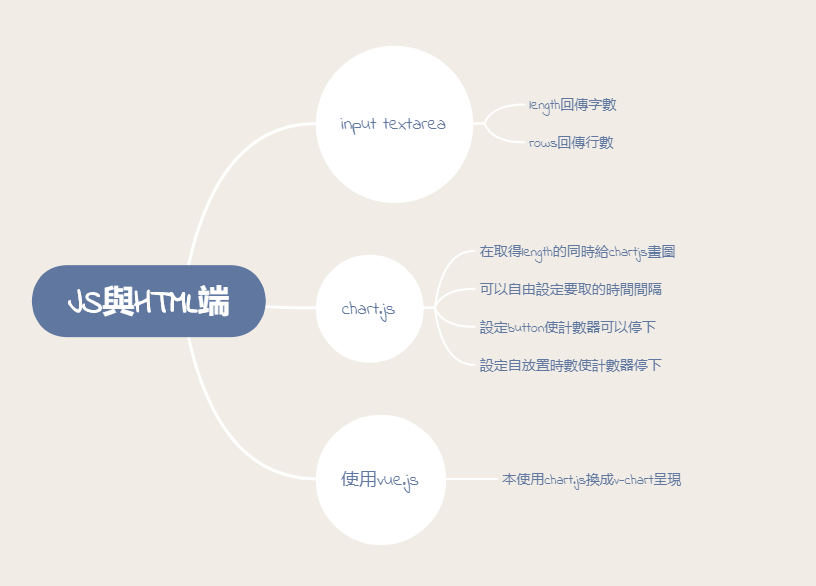
\includegraphics[width = .8\textwidth]{c5C4T4t.png}
\begin{figure}[H] %H为当前位置,!htb为忽略美学标准,htbp为浮动图形
		\centering %图片居中
		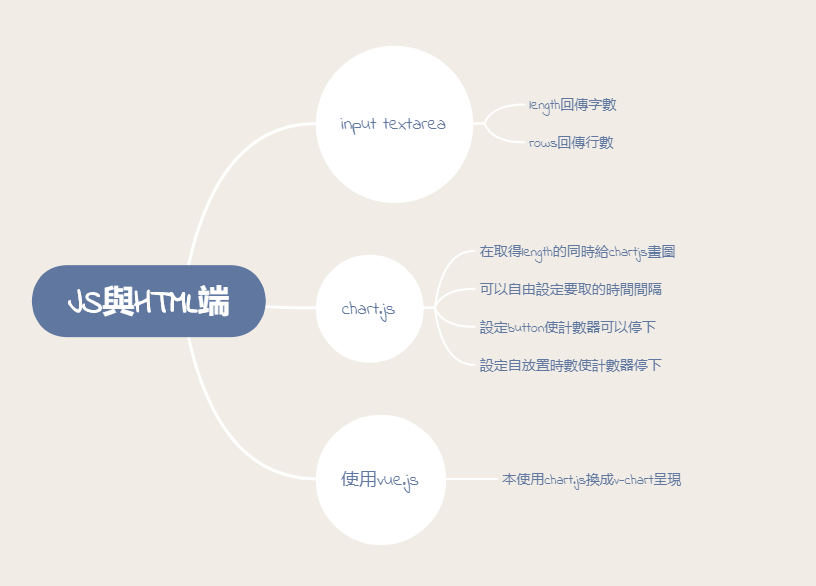
\includegraphics[width=0.7\textwidth]{1.png} %插入图片,[]中设置图片大小,{}中是图片文件名
		\caption{從JS、HTML以及Vue所打造的前端網頁中擷取資料} %最终文档中希望显示的图片标题
		\label{Fig.3.1} %用于文内引用的标签
\end{figure}
\subsection{模擬平台}
\begin{itemize}
	\item 目前所使用的解題平台雛形,其作答畫面如下圖所示。
	\begin{figure}[H]
		\centering
		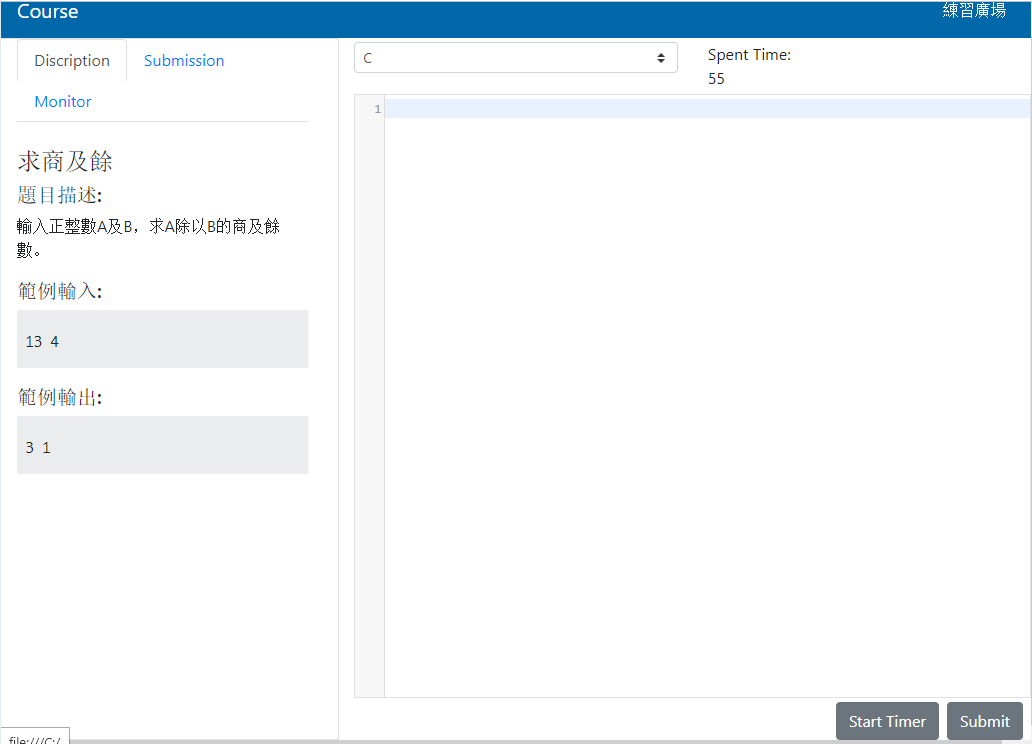
\includegraphics[width=0.7\textwidth]{web_part.png}
		\caption{模擬平台介面}
		\label{Fig.3.2}
	\end{figure}
	\item 功能:\\
	\begin{enumerate}[1.]
		\item 左方:顯示使用者正在作答的題目,包括輸入輸出的範例,供使用者了解目前作答的題目。使用者投稿之後,系統會自動切換至Submission頁籤,這個頁籤是評判伺服器進行評測之後所回傳的結果,包括答題正確狀況以及程式碼的格式檢查結果。
		\item 右上計算時間讀秒:右上的計時器記錄使用者所耗費的作答時間,每隔一定時間,系統會自動擷取使用者所輸入的內容,連同當時耗費的時間傳送到Firebase資料庫中。
		\item 右下的Stop Timer:暫停計時和傳送資料,目前做為除錯用途。
	\end{enumerate}
\end{itemize}

\subsection{基本統計資訊}
\begin{itemize}
	\item 字數與行數的判讀與計算\\
	取得使用者輸入的程式碼內容後,使用以下JS指令計算總共輸入的字數和行數:

\begin{lstlisting}[caption=js字數與行數的判讀與計算]
// code = 使用者輸入的程式碼內容
chars = code.length;
lines = 1+code.match(/\r?\n|\r/g).length; // 使用正規表達式尋找換行符號
\end{lstlisting}
此處用來判斷行數據的方法,主要是偵測使用者所用到的換行符號。如果使用者的程式碼文字中有其他的換行文字,可能會造成誤差。這個部份,未來可以使用鍵盤偵測來進行改良。計算出來的統計數字會使用HTML頁面顯示出來。

\item 時間的判讀與計算\\
目前用來擷取資料的方法主要是透過JS的setInterva函式,setInterval函式可以每隔一個設定時間不斷重覆執行特定的任務,在這裡主要是擷取使用者的作答內容。\cite{name20}
應該注意的一點,當作答結束之後,或者停止擷取資料之後,也要把setInterval所建立的程序清除掉,否則它會一直留在網頁中不斷執行,有可能會造成系統的問題。
擷取到的資料被傳送到Firebase中,可以用來做接下來的數據分析。
\end{itemize}
\subsection{輸出}
\begin{itemize}
	\item 即時監測圖:\\
	使用者的輸入內容和時間傳送到firebase的資料庫之後,會自動傳送收據更新的訊息到監控程式,監控程式的目的是顯示同學作答的一些統計資訊。
	目前數據的監測先選定一位同學為主,同學作答的時間,與輸入的字數和行數會使用圖形顯示出來。這邊使用了chart.js與vue.js來顯示前端的數據圖形。
	(圖3.3)
	\begin{figure}[H] %H为当前位置,!htb为忽略美学标准,htbp为浮动图形
		\centering %图片居中
		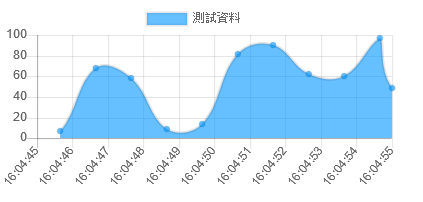
\includegraphics[width=0.7\textwidth]{3.png} %插入图片,[]中设置图片大小,{}中是图片文件名
		\caption{作答統計資訊範例} %最终文档中希望显示的图片标题
		\label{Fig.3.3} %用于文内引用的标签
	\end{figure}
呈現的統計圖每隔一段時間會隨著新的擷取資料而自動更新。資料擷取的時間間隔目前設定每秒一次,但可以隨著需要而做更改。圖表的 X 軸為時間,Y 軸為字數與行數。\\
	\item 影片輸出:\\
	除了進行數據監測及圖形繪製,另外也可以模擬同學作答過程的畫面,這部份一樣是Firebase傳送的數據更新資料,以畫面顯示當时同學的畫面,進行即時的監控。另外也可以根據這些資料,自動生成模擬同學作答畫面的影片,供教師或研究人員參考。
\end{itemize}
\section{基礎數據分析}
	\begin{figure}[H] %H为当前位置,!htb为忽略美学标准,htbp为浮动图形
	\centering %图片居中
	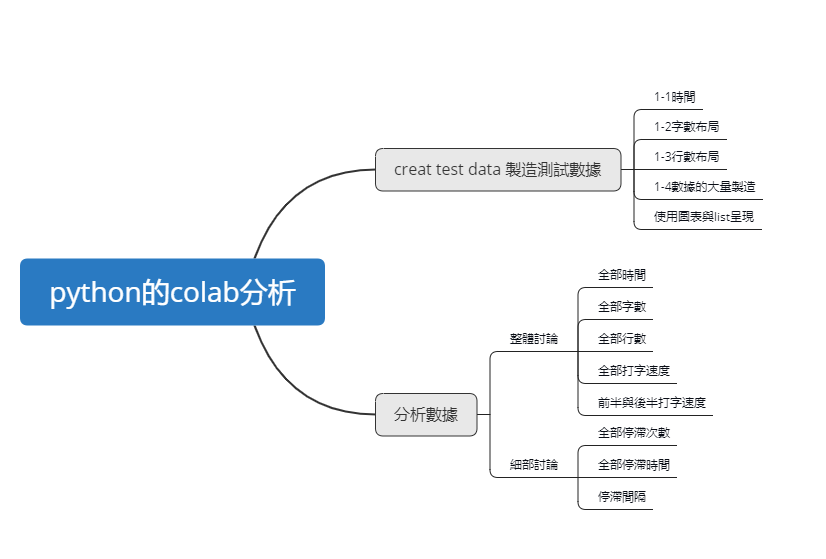
\includegraphics[width=0.7\textwidth]{2.png} %插入图片,[]中设置图片大小,{}中是图片文件名
	\caption{分析系統架構} %最终文档中希望显示的图片标题
	\label{Fig.3.4} %用于文内引用的标签
	\end{figure}
除了即時監測使用者的輸入狀況,我們也對收錄的資料做了一些基礎的統計分析,目前分析的內容包括:
1. 個別同學做一題的總時間分析,以及全部同學的平均作答時間
2. 停頓分析:如果作答的內容一直沒有改變,表示這位同學可能在某處卡住了。可以先找出停頓的位置,未來可以據此做更進一步的分析處理。

\subsection{模擬測試數據}
\subsubsection{討論數據的特徵}
圖(3.5)是典型作答過程的統計數字,因為是打字數與時間的關係,所以數據自然是漸進式的。圖中佔據面積比較大的部份為字數統計,下方面積比較小的部份為行數。
由於研究過程中,測試的作答平台尚未完整,因此除了採集一些個別少量的數據之外,先使用模擬產生的數據來進行分析,以觀察分析模組是否能正常運作。
	\begin{figure}[H] %H为当前位置,!htb为忽略美学标准,htbp为浮动图形
	\centering %图片居中
	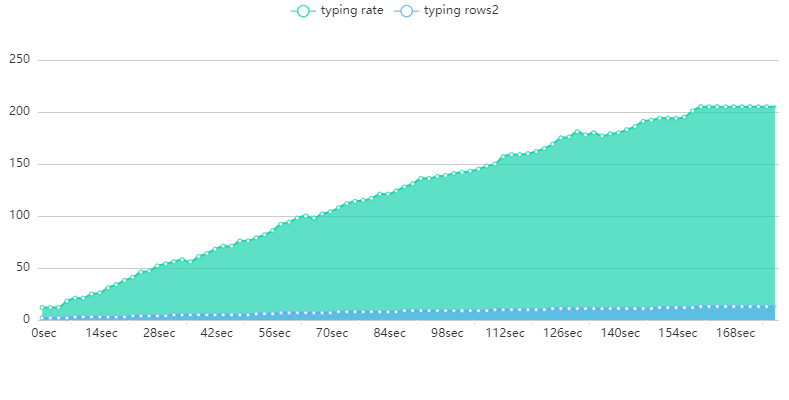
\includegraphics[width=0.7\textwidth]{4.png} %插入图片,[]中设置图片大小,{}中是图片文件名
	\caption{執行結果漸增圖} %最终文档中希望显示的图片标题
	\label{Fig.3.5} %用于文内引用的标签
	\end{figure}

在產生模擬數據之前,先討論一些作答數據的特徵和假設:
1. 規定時間區間:一個班級同學做同一題目,大家所完成的時間會有差別,可以規定自做的數據時間(ex:15分~1小時),而30分鐘可能是大部分人完成的時間,15分是做得快的,50分以上是做得慢的。
2. 作答字數:基本上整體分佈要像上圖一樣呈漸進增加的趨勢,但每位同學的字數增長速度可能不同,停頓的地方可能也不同,字數的增長也要設定一個合理的區間。
3. 作答行數:理論上越多字的越多行,但還是要在合理的範圍,不能生成太多行數。

\subsubsection{規定格式}
在統計圖(3.5)中包括三個欄位:時間、字數與行數。為了方便後續的分析,我們採用陣列的方式來儲存模擬數據。基本上模擬數據為三欄的陣列,其列數為模擬製造的記錄個數,以下分三部分說明各欄位數據的構成。
\subsubsection{時間欄位}
由於網頁程式擷取作答內容的時間間隔是固定的,因此為時間欄位為固定間隔的時間序列。(圖3.6)
	\begin{figure}[H] %H为当前位置,!htb为忽略美学标准,htbp为浮动图形
	\centering %图片居中
	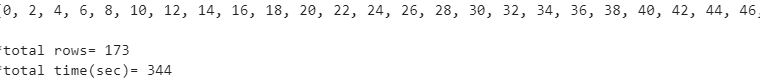
\includegraphics[width=0.7\textwidth]{3_2_1_3.png} %插入图片,[]中设置图片大小,{}中是图片文件名
	\caption{網頁程式執行結果圖} %最终文档中希望显示的图片标题
	\label{Fig.3.6} %用于文内引用的标签
	\end{figure}
每位同學在撰寫時所完成的時間也不相同,在產生數據時規定上下界,如同規定最快完成與最慢完成所需花費的時間。

\begin{lstlisting}[language=Python,caption=時間欄位的模擬數據]
data_up = 180
data_down = 500  #可以自行規定秒數區間
random_data = random.randint(data_up,data_down) #這是秒數
r1 = list(range(0,random_data,2)) #r1是第一部分時間陣列的部分
print(r1)
r_row1=len(r1)
r_row2=r1[-1]
print("\n*total rows=",r_row1,)
print("*total time(sec)=",r_row2) #計算random的格數與秒數(秒數為最後一個數據)
\end{lstlisting}
使用random函數進行最大秒數的選擇,後頭的第二與第三數據產生也大量地使用random函數。

\subsubsection{模擬字數}
這個部份可以說是最重要和最複雜的部份,因為使用者作答過程可能會有很多不同的變化。最初的構想的是使用者
作答的字數每次取樣都會不停地增加,但每次增加的字數不同,先使用亂數來模擬增加的字數。

\begin{lstlisting}[language=Python,caption=作答字數的模擬數據]
a = random.randint(0,10)
b = random.randint(a,20)
c = random.randint(b,30)
d = random.randint(c,40)
e = random.randint(d,50)
f = random.randint(e,60)
g = random.randint(f,70)
h = random.randint(g,80)
print(a,b,c,d,e,f,g,h)
\end{lstlisting}

如此,此程式所呈現的結果是(8 13 21 34 38 59 64 67),當然每執行一次都不同。
但這樣一來,使用者作答的字數會無止盡的增加,但這樣的方式沒有辦法反映使用者遇到不會的地方而卡住的情況,
所以要加入"使用者在思考"的停頓狀況,也就是會要維持同樣的字數一段時間。

除了停頓之外,使用者也有可能打錯字而按下倒退(Backspace)鍵,另外也可能使用了選擇和刪除的功能,
所以整體的數據並不會一路平滑的增加,必須在模擬數據中加上這些考量才比較合理。

於是我們新增三個模擬參數,分別用來處理增加、停頓、倒退和刪除的不同情況,
先使用random函數決定使用者可能的三個動作,而在增加與減少的時候,
數據的變化量是不均勻的,此部分一樣使用random函數來實現,如圖3.7所示。
\begin{figure}[H] %H为当前位置,!htb为忽略美学标准,htbp为浮动图形
	\centering %图片居中
	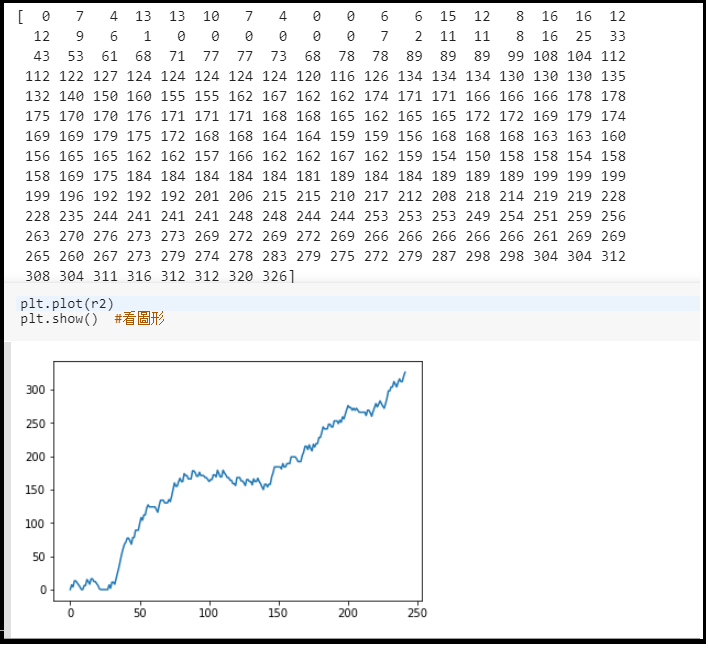
\includegraphics[width=0.7\textwidth]{3_2_1_4.png} %插入图片,[]中设置图片大小,{}中是图片文件名
	\caption{作答字數的模擬改良} %最终文档中希望显示的图片标题
	\label{Fig.3.7} %用于文内引用的标签
\end{figure}

\subsubsection{模擬行數}
第三部分為作答行數,這部分與字數息息相關,但是換行的判斷比較簡單,一般只要觀察原始程式碼是否有換行符號即可得知。此處是製
造出0,0,0,1,1,1,2,2,2,3,3,3,3,3,3,3,4,4,4,.....之類的漸增數列,但是增加的幅度遠比第二部分的字數還要緩慢許多。(圖3.8)
	\begin{figure}[H] %H为当前位置,!htb为忽略美学标准,htbp为浮动图形
	\centering %图片居中
	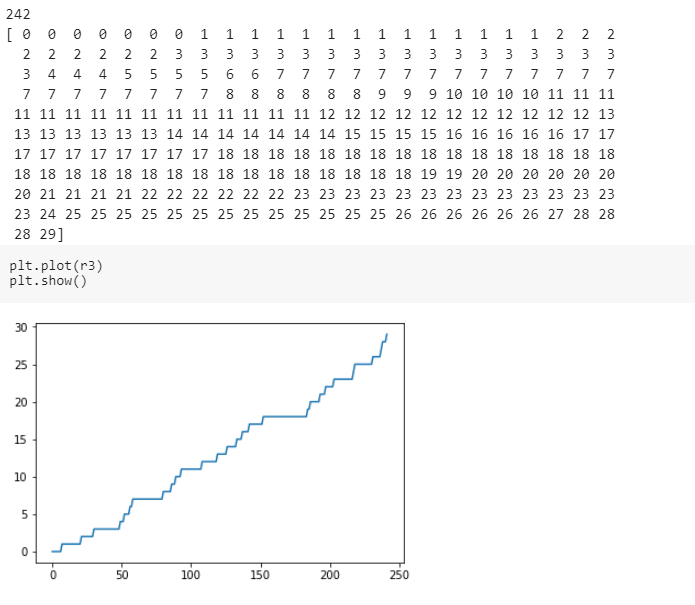
\includegraphics[width=0.7\textwidth]{3_2_1_5.png} %插入图片,[]中设置图片大小,{}中是图片文件名
	\caption{作答行數的數據模擬} %最终文档中希望显示的图片标题
	\label{Fig.3.8} %用于文内引用的标签
	\end{figure}

\subsection{數據分析}
\subsubsection{單組數據整體分析}
\begin{itemize}
	\item 可從最為直觀的記算所有數據的平均速度或是平均字數為基礎,在加上停頓點的分析。
	因為把數據設計成三欄的陣列,在分析步驟可以很容易抓到要的數據進行運算。
	\item 在陣列上最容易計算的如:作答時間、做答完畢字數、做答完畢(圖3.9)
	\begin{figure}[H] 
		\centering 
		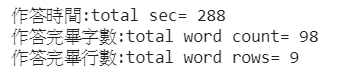
\includegraphics[width=0.5\textwidth]{3_8.png} 
		\caption{整體結果} 
		\label{Fig.3.9} 
	\end{figure}
	然後往下延伸計算的數據,如平均做答速度、前半作答速度、後半作答速度;在速度的計算上分兩部分是因為如果只有一個均速可能在比較上會有較大誤差,因此做多個速度的比較數據會更佳。(圖3.10)
	\begin{figure}[H] 
		\centering 
		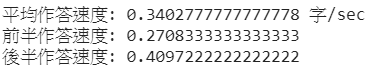
\includegraphics[width=0.5\textwidth]{3_9.png} 
		\caption{整體速度結果} 
		\label{Fig.3.10} 
	\end{figure}
	\item 收集這些速度的數據在之後比較多組,也就是多個同學更能知道每個人的打字速度,除了分析打字的字數外速度也可以加入進行細部分的分析。
\end{itemize}

\subsubsection{單組數據細部分析}
\begin{itemize}
	\item 除了單組數據的整體分析,最總體的數據與平均時間外,打字的停滯點也是至關重要。
	\item 要找出數組中的斷點若是直接觀察是非常容易的,如(圖3.10)
		\begin{figure}[H] 
		\centering 
		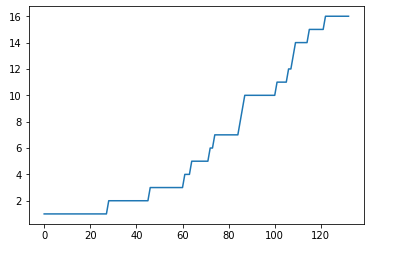
\includegraphics[width=0.7\textwidth]{3_10.png} 
		\caption{示例圖片} 
		\label{Fig.3.11} 
	\end{figure}
	若是看到打字沒有增加,在圖中是平行線段,就代表動作停滯、維持同一字數。
	\item 找出停滯部分本研究所使用方法是,使陣列的後項數據剪去前項數據,並且判斷此數據值若是正數,則判斷增加;若是0,判斷停滯;若是負數,判斷刪除倒退。
	可將此判斷數據化存成另一陣列,在此以下稱trend陣列。\\
	1. 後項減去前項為正:打字字數增加,1表示\\
	2. 後項減去前項為零:打字字數不變,0表示\\
	3. 後項減去前項為負:打字字數減少,-1表示\\
	將判斷後1,0,-1的值存入trend陣列,故此陣列為三個元素組成,且比原本數據的陣列值少一,因為trend陣列是原陣列間隔中的差分。(圖3.12)
		\begin{figure}[H] 
		\centering 
		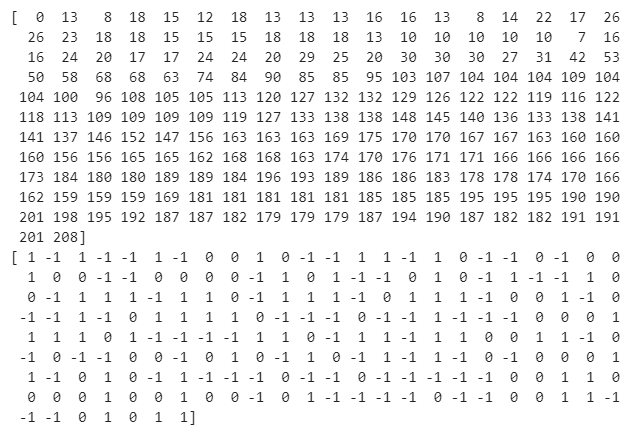
\includegraphics[width=0.7\textwidth]{3_11.png} 
		\caption{trend陣列輸出} 
		\label{Fig.3.12} 
	\end{figure}
	上半部陣列為原數據的陣列,字數遞增;下半部為使用1,0,-1判斷產生的trend陣列。
	如此便很清楚的看出,0是使用者停下的部分,之後能從0所停頓的時間長度,或是停頓所發生的次數判斷分析。
	\item 除了把trend陣列顯示外,若能畫圖更能掌握此陣列數據的特徵。(圖)點狀圖
	\begin{figure}[H] 
		\centering 
		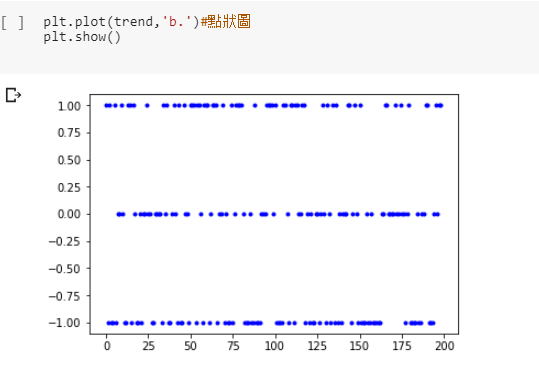
\includegraphics[width=0.7\textwidth]{3_12.png} 
		\caption{trend點狀圖} 
		\label{Fig.3.13} 
	\end{figure}
	(圖)圓餅圖
	\begin{figure}[H] 
		\centering 
		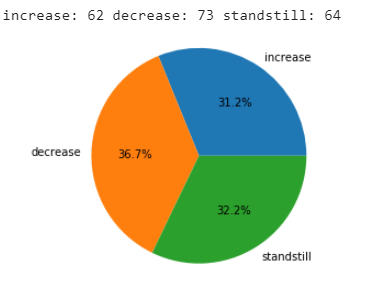
\includegraphics[width=0.7\textwidth]{3_13.png} 
		\caption{trend圓餅圖} 
		\label{Fig.3.14} 
	\end{figure}
\item 製做點狀圖或是圓餅圖可以顯示使用者停頓、打字或是刪除的密集程度。不過此處若是希望只看停頓處的地方,於是在多新增一個新的陣列,以下稱trend2。trend2是把0的元素抓出,把0換成1;因此trend2數據便只有0與1數值。
\item 部分程式:
\begin{lstlisting}[language=Python,caption=python數據trend2]
#len(trend)#trend的隔數 大約表示時間的1/2
trend2=np.zeros(len(trend),int)
for j in range (0,len(trend2)):
	if (trend[j]!=0):
		trend2[j]=0
	else :
		trend2[j]=1
print(trend)
print(trend2)#trend2是trend的停頓部分
\end{lstlisting}
將trend與trend2顯示(圖3.15)
	\begin{figure}[H] 
	\centering 
	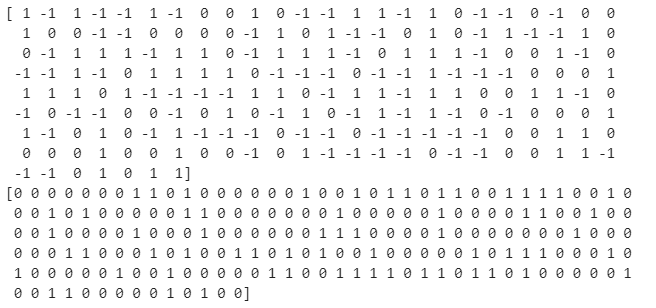
\includegraphics[width=0.7\textwidth]{3_14.png} 
	\caption{trend2輸出} 
	\label{Fig.3.15} 
\end{figure}
\newpage
如此只剩0與1兩個元素的trend2陣列畫成柱狀圖觀察,如同條碼的形狀。(圖3.16)其中線條就是使用者停頓處。
	\begin{figure}[H] 
	\centering 
	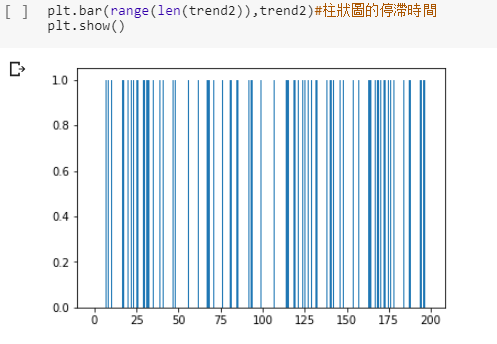
\includegraphics[width=0.7\textwidth]{3_15.png} 
	\caption{trend2條碼狀方圖} 
	\label{Fig.3.16} 
\end{figure}
\item 最後一個圖做分區的統計,這裡計算trend2陣列1的出現次數,並且做分區的統計次數。
分區的分法是察看trend2的全部元素個數,並且分成五等分,在一個個部分統計停頓的出現次數,例如若有200數據,則第一部份統計1出現個數為0~50組,第二部分統計為50~100,以下類推。(圖3.17)
	\begin{figure}[H] 
	\centering 
	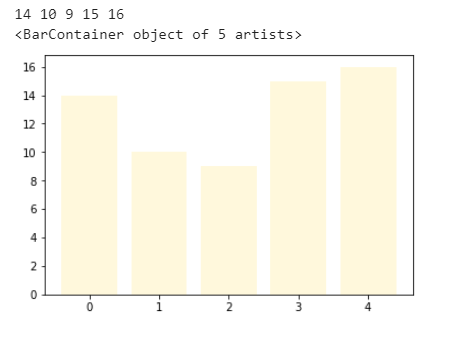
\includegraphics[width=0.7\textwidth]{3_16.png} 
	\caption{trend2分區圖} 
	\label{Fig.3.17} 
\end{figure}
不過如此計算的密度為強制分區,可能無法把密度情況很好的呈現出來,此部份討論於結果部份做詳細討論檢討。
\end{itemize}
\subsubsection{多組數據}
\vspace*{-4mm}
以上分析都是只使用一組數據分析與統計的結果,若要在此基礎上擴增成多數據的分析,則需要進行更多數據的製造與集合分析,所以以上的步驟需要進行多次。
如此進行多次迴圈,此迴全次數可以自行修改。(圖3.18)為設定10次所呈現之全部格數與全部時間。
\begin{figure}[H] 
	\centering 
	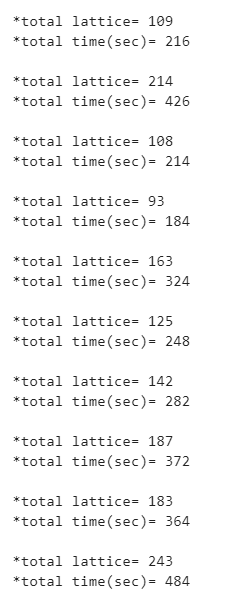
\includegraphics[width=0.4\textwidth]{3_17.png} 
	\caption{多組數據} 
	\label{Fig.3.18} 
\end{figure}

